% 第 25 题正三棱柱 ABC-A1B1C1：源为嵌入位图（869×1233），顶点按源 400 dpi 渲染实测
% （1 单位 = 1 pt 源页尺寸；页面坐标 y 向下换算 Y = 580 − y_page）。
% 照源线型：实线 6 段（AB、AA1、BB1、A1B1、A1C1、B1C1，上底边 A1B1 未画虚线）；
% 虚线 4 段（C1C 后侧棱、CA 与 CB 底后两边、BC1——题目所求异面直线之一，源内即画为虚线）。
% 源内竖方向未缩短（侧棱 92.8pt / 底边 69.5pt = 1.335 ≈ 题设 4/3），C 点退深约 45°。
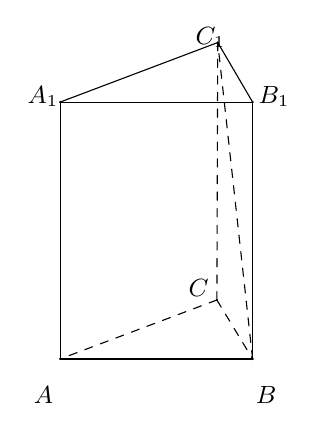
\begin{tikzpicture}[line cap=round,line join=round,font=\small,x=0.03515cm,y=0.03515cm]
% ===== 实线（6 段）=====
\draw (444.0,23.4)--(513.5,23.4);    % AB（底前边）
\draw (444.0,23.4)--(444.0,116.2);   % AA1（左侧棱）
\draw (513.5,23.4)--(513.5,116.2);   % BB1（右侧棱）
\draw (444.0,116.2)--(513.5,116.2);  % A1B1（上底边，源内未画虚线）
\draw (444.0,116.2)--(500.9,137.7);  % A1C1（上底左后边）
\draw (513.5,116.2)--(500.9,137.7);  % B1C1（上底右后边）
% ===== 虚线（4 段）=====
\draw[dashed] (500.9,137.7)--(500.6,44.7);  % C1C（后侧棱）
\draw[dashed] (500.6,44.7)--(444.0,23.4);   % CA（底后左边）
\draw[dashed] (500.6,44.7)--(513.5,23.4);   % CB（底后右边）
\draw[dashed] (513.5,23.4)--(500.9,137.7);  % BC1（所求异面直线之一）
% ===== 顶点实心点（源内六顶点均带小点，直径约 0.9pt）=====
\fill (444.0,23.4) circle[radius=0.45pt];
\fill (513.5,23.4) circle[radius=0.45pt];
\fill (500.6,44.7) circle[radius=0.45pt];
\fill (444.0,116.2) circle[radius=0.45pt];
\fill (513.5,116.2) circle[radius=0.45pt];
\fill (500.9,137.7) circle[radius=0.45pt];
% ===== 标签（照源墨迹中心，显式坐标）=====
\node[anchor=center,inner sep=0] at (438.0,10.5) {\(A\)};
\node[anchor=center,inner sep=0] at (518.4,10.5) {\(B\)};
\node[anchor=center,inner sep=0] at (494.0,49.0) {\(C\)};
\node[anchor=center,inner sep=0] at (437.8,118.3) {\(A_{1}\)};
\node[anchor=center,inner sep=0] at (521.3,118.3) {\(B_{1}\)};
\node[anchor=center,inner sep=0] at (498.3,139.5) {\(C_{1}\)};
\end{tikzpicture}
